\section{Проектирование и разработка программного средства}

\subsection{Архитектура программного средства}

Процесс разработки программного обеспечения для голосового помощника для одноплатного компьютера требует внимательного подхода к проектированию, с учетом особенностей работы на ограниченных ресурсах и необходимости обеспечения масштабируемости. Как показано на рисунке~\ref{fig:class_diagram}, для решения этих задач был выбран объектно-ориентированный подход, обеспечивающий четкое разделение функциональности на независимые компоненты.

\begin{figure}[H]
	\centering
	\fbox{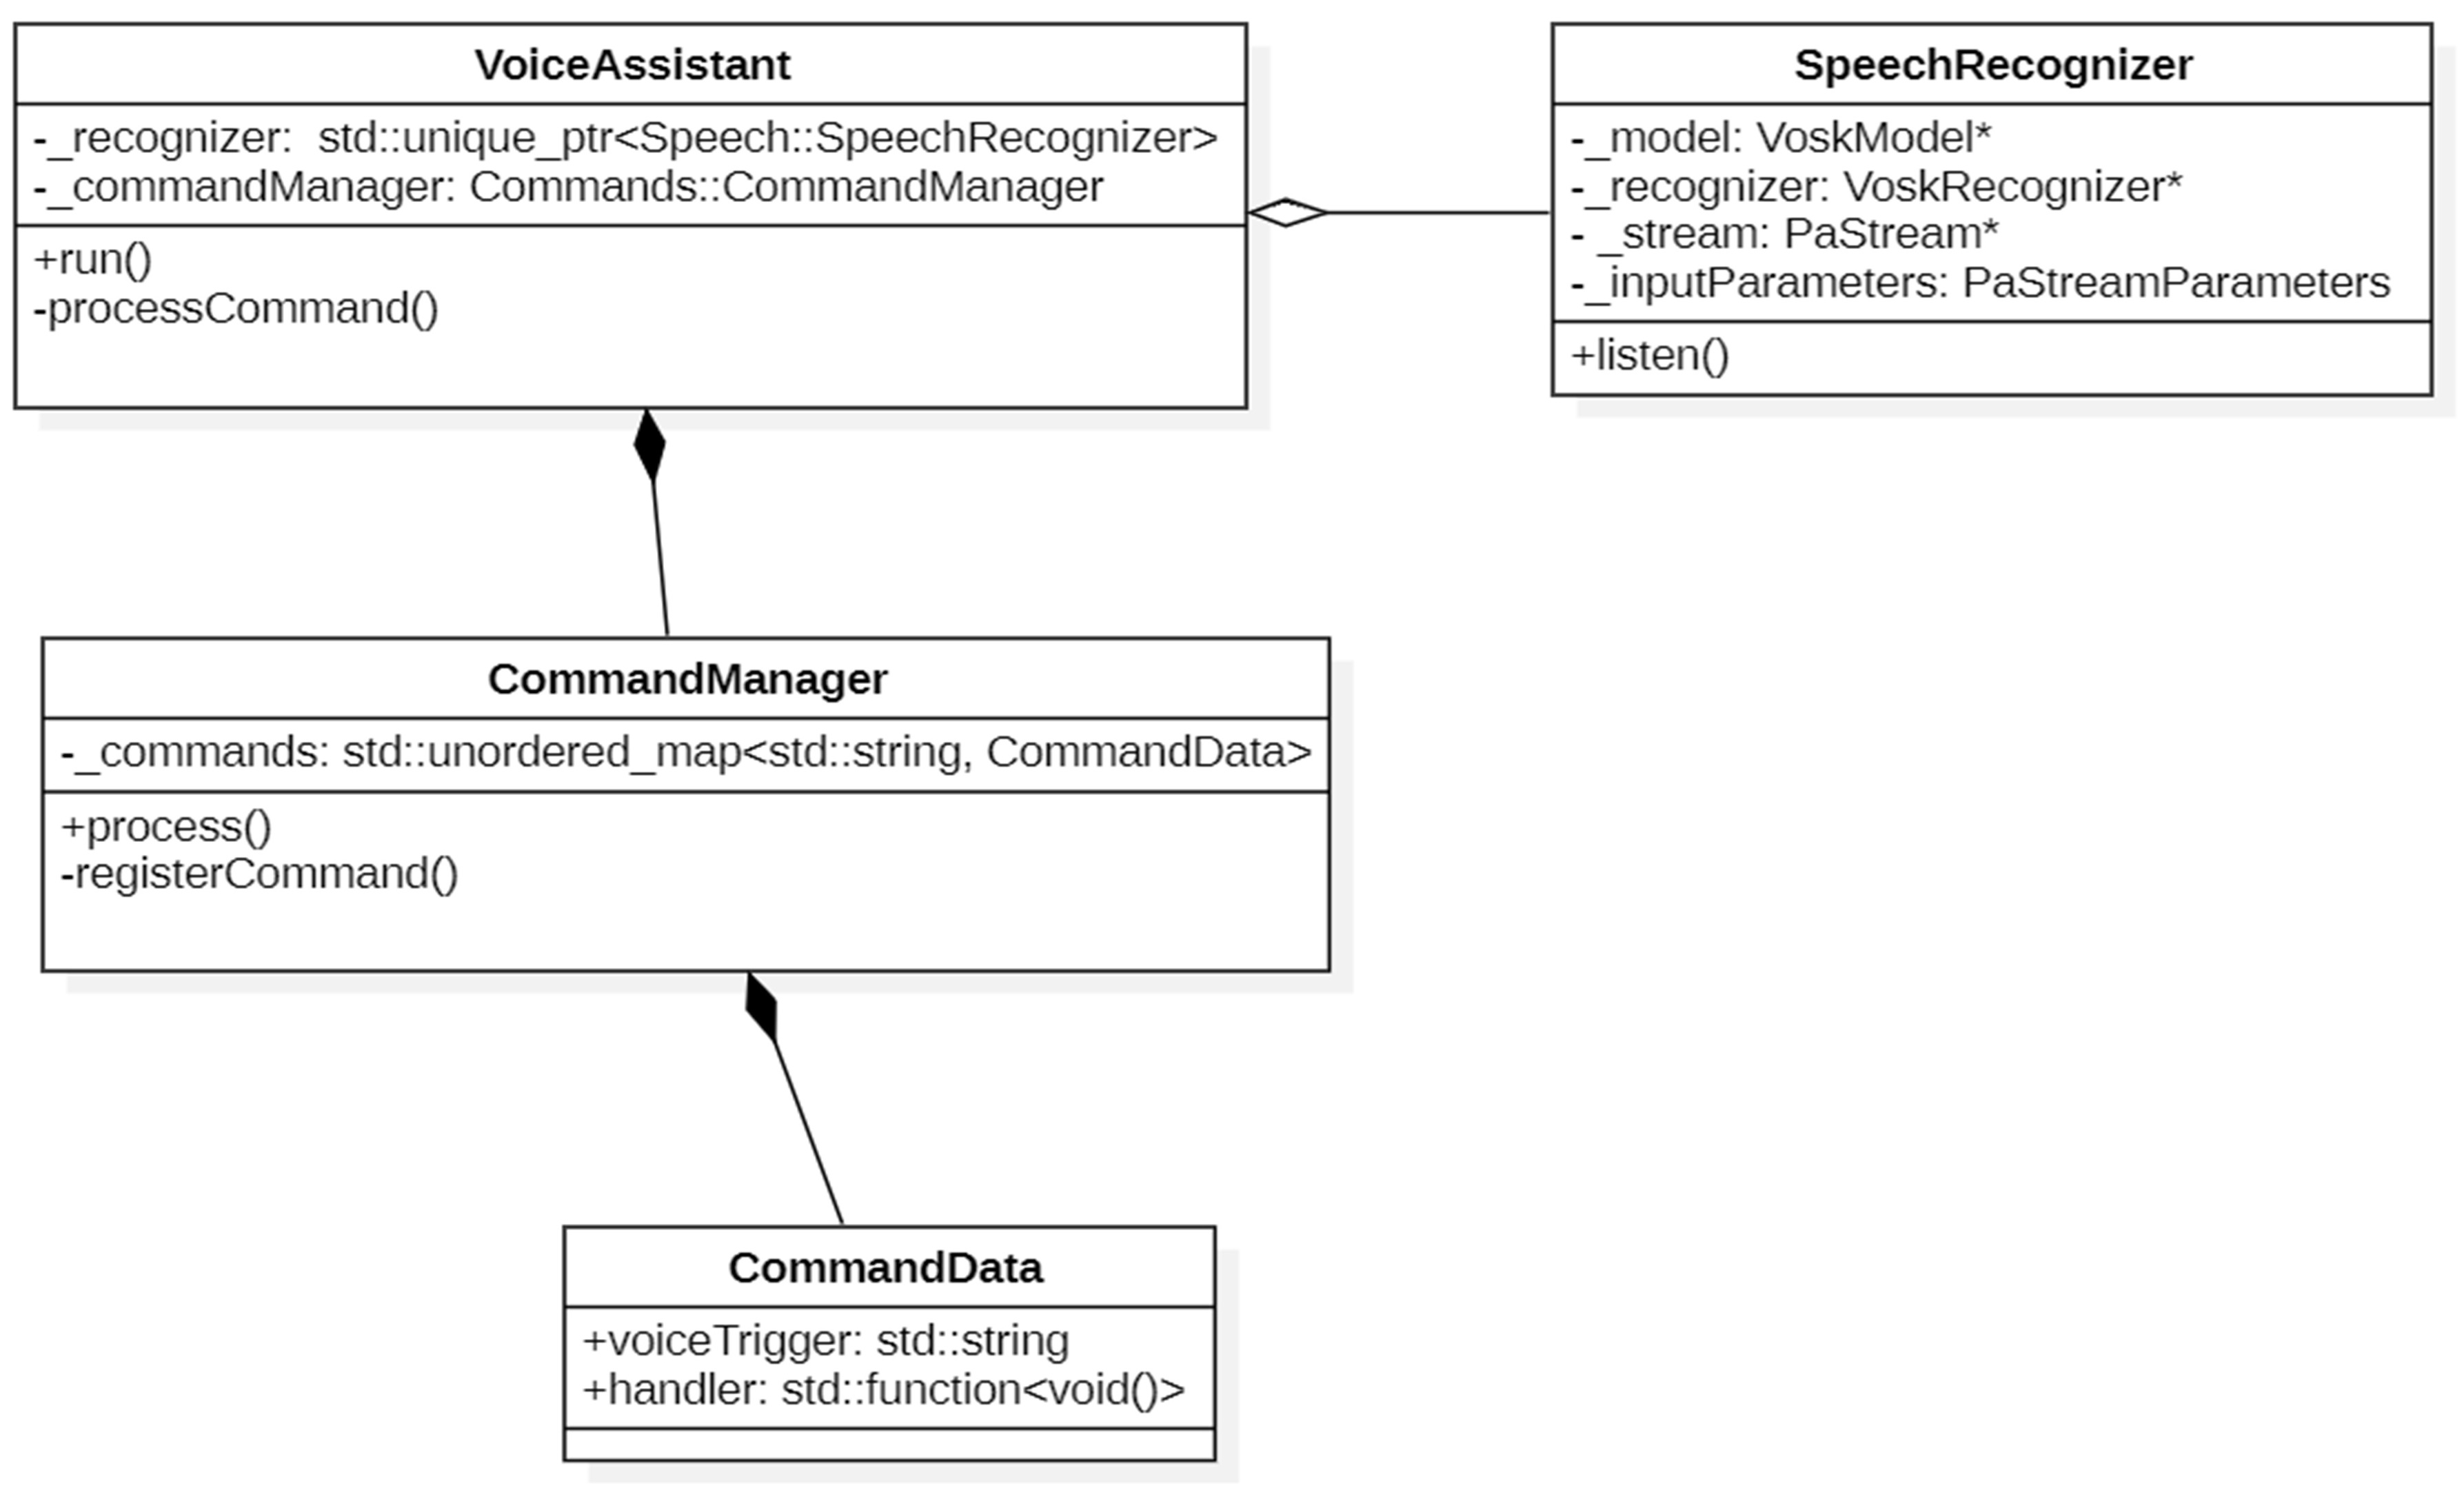
\includegraphics[scale=0.25]{class_Diagram.jpg}}
	\caption{Диаграмма классов}
	\label{fig:class_diagram}
\end{figure}
На рисунке~\ref{fig:class_diagram} показано что программное средство состоит из следующих основных компонентов:

\begin{itemize}
	\item {Core::VoiceAssistant} -- центральный компонент, управляющий жизненным циклом голосового помощника. Он отвечает за инициализацию всех необходимых модулей и запуск основного цикла обработки команд.
	
	\item {Speech::SpeechRecognizer} -- модуль распознавания речи, использующий библиотеку Vosk и PortAudio для захвата и анализа аудиопотока с микрофона.
	
	\item {Commands::CommandManager} -- отвечает за регистрацию голосовых команд и выполнение соответствующих обработчиков при их распознавании.
\end{itemize}

Взаимодействие между компонентами организовано следующим образом: VoiceAssistant инициализирует экземпляр SpeechRecognizer, а затем в бесконечном цикле получает голосовой ввод, преобразованный в текст. Полученный текст передается в CommandManager, который анализирует его и при обнаружении соответствующей команды вызывает заранее зарегистрированную функцию-обработчик.

Такой подход позволяет легко расширять систему, добавляя новые голосовые команды, не затрагивая существующую логику работы помощника.

Представленная архитектура с модульным разделением компонентов позволяет системе поддерживать различные сценарии взаимодействия. На рисунке \ref{fig:use_case_diagram} показана диаграмма вариантов использования, иллюстрирующая основные функциональные возможности голосового помощника и взаимодействие с пользователями разных категорий.

\begin{figure}[H]
	\centering
	\fbox{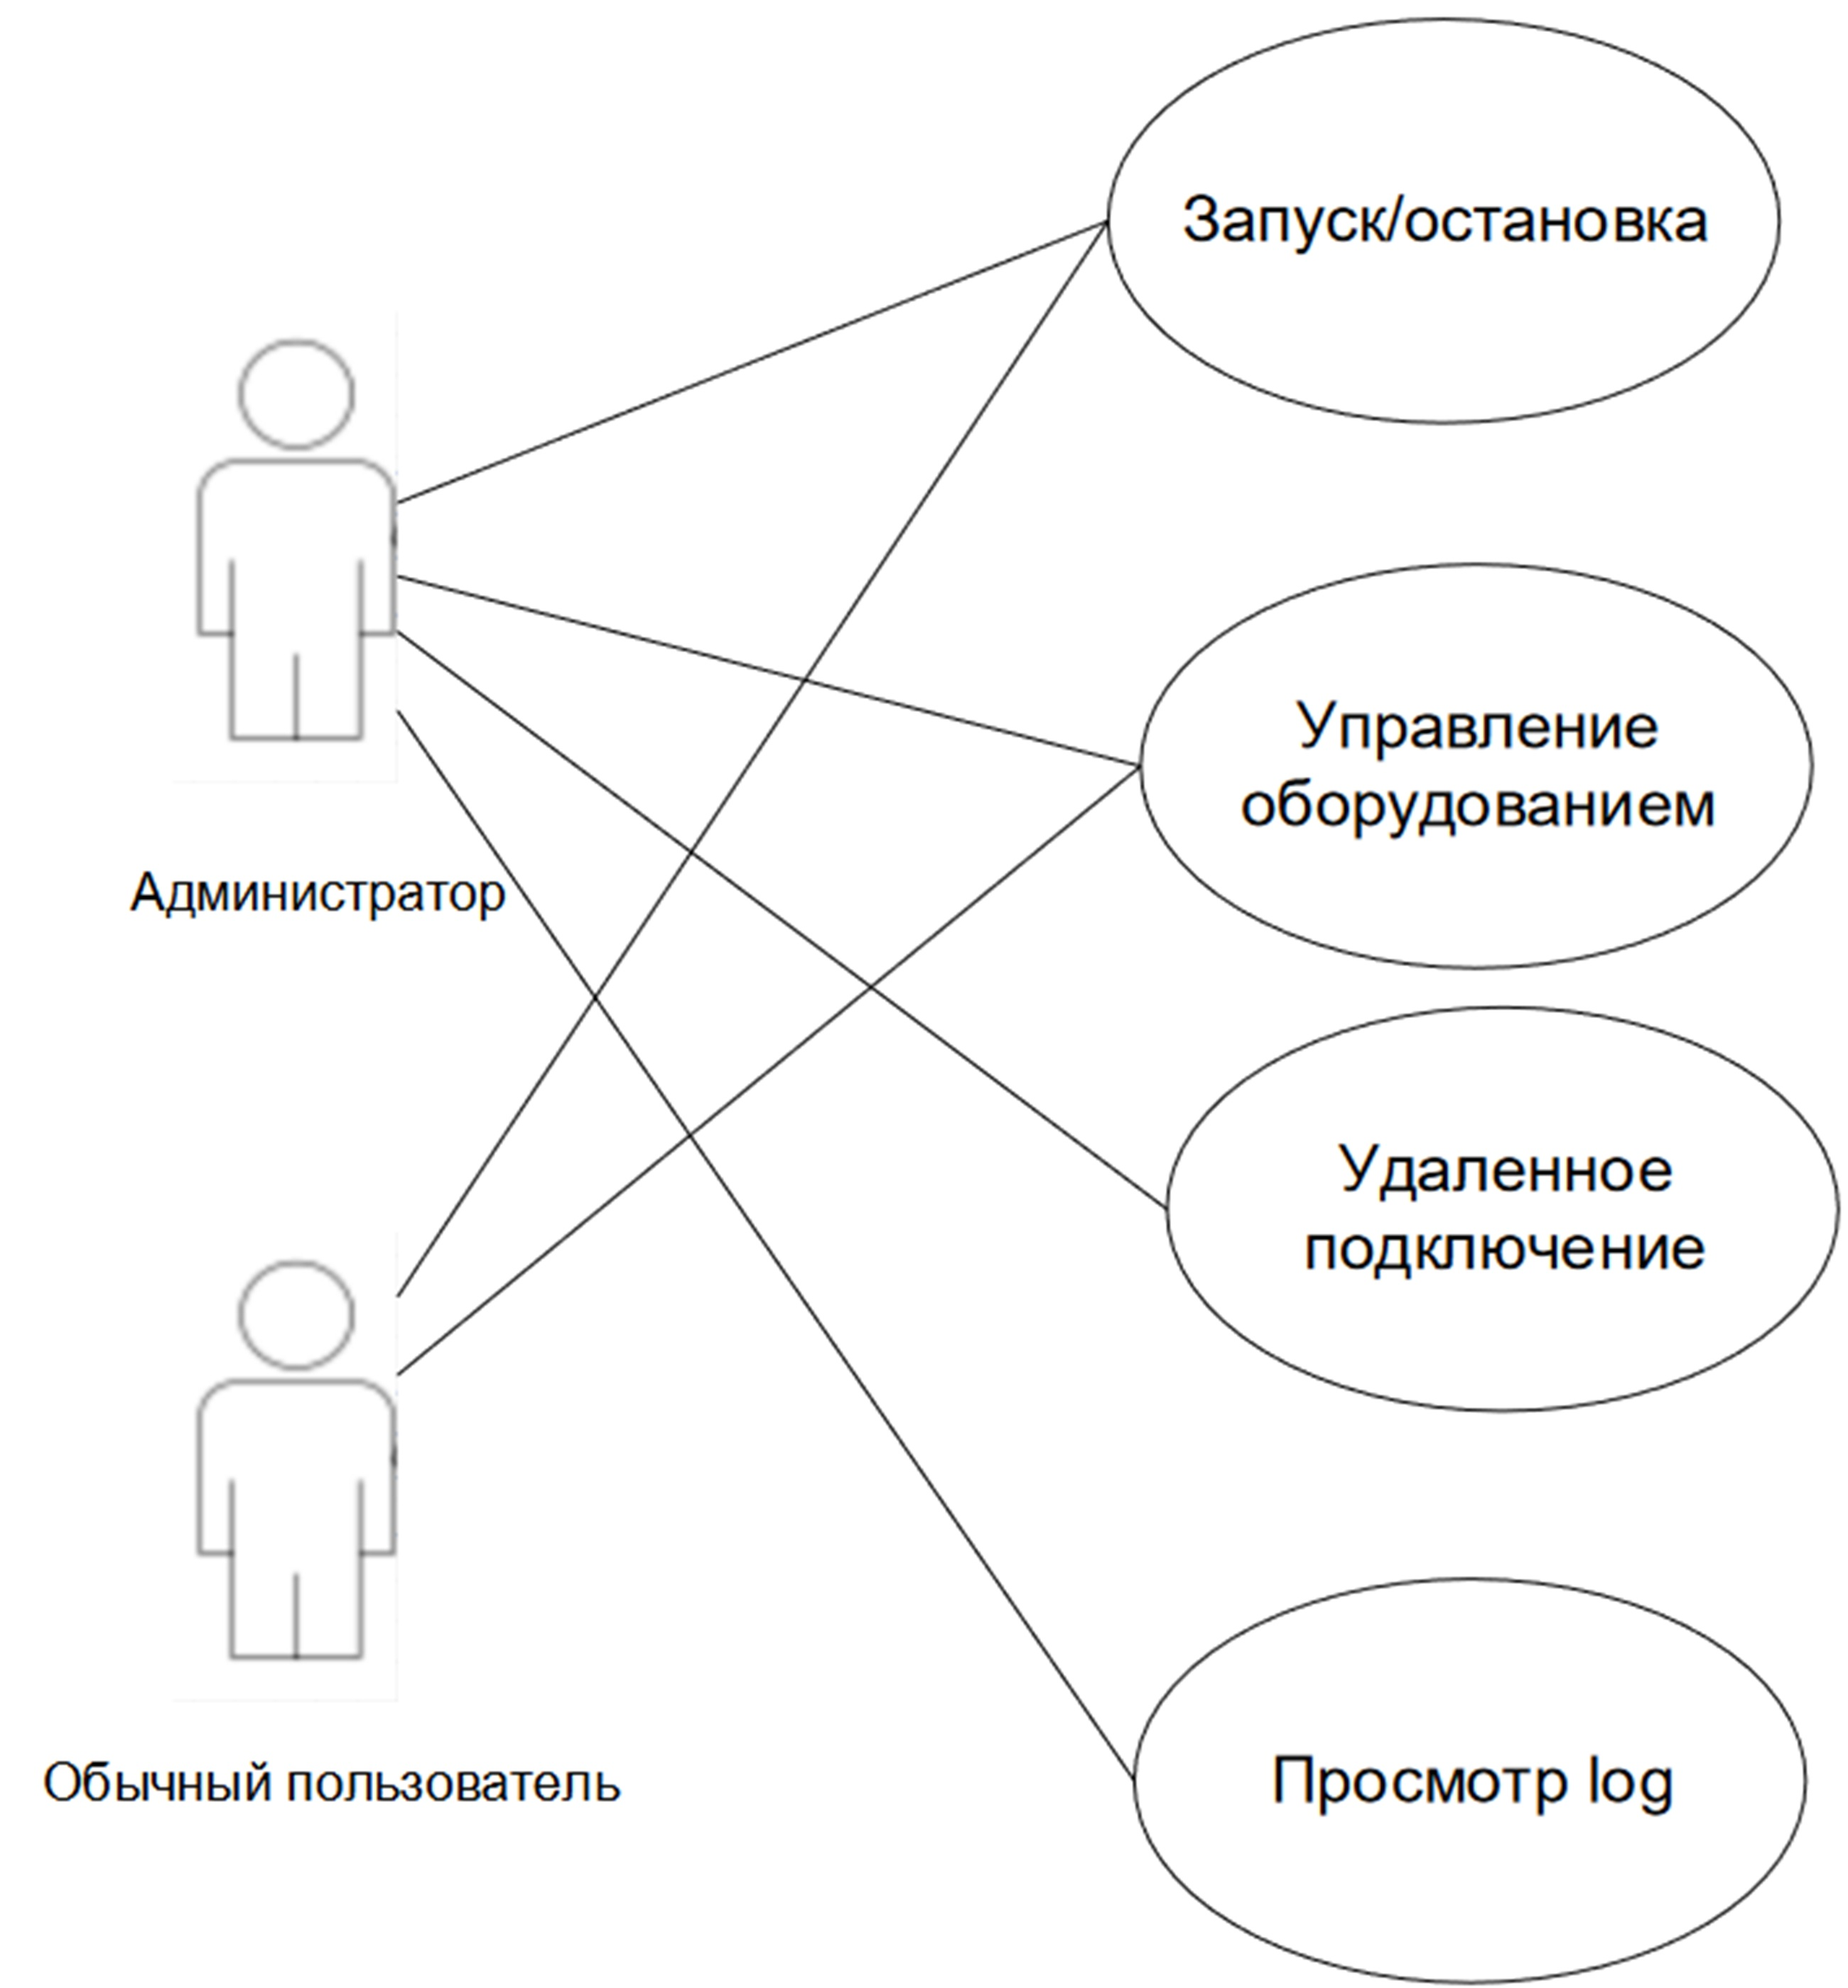
\includegraphics[scale=0.3]{use_Case_Diagram.jpg}}
	\caption{Диаграмма вариантов использования}
	\label{fig:use_case_diagram}
\end{figure}

Диаграмма вариантов использования иллюстрирует ключевые функциональные возможности системы, разделенные по категориям пользователей. Основной функционал доступен всем пользователям и включает базовые операции: запуск/остановку системы и управление подключенным оборудованием. Эти функции представляют собой ядро системы, необходимое для повседневной работы с голосовым помощником.

Для администраторов предусмотрен расширенный набор возможностей, включающий удаленное подключение к системе и просмотр системных логов. Эти функции предназначены для технического обслуживания, мониторинга работы системы и устранения неполадок.

Система четко разделяет пользователей на две категории:
\begin{itemize}
	\item обычные пользователи -- работают только с базовым функционалом;
	\item администраторы -- обладают полным доступом ко всем возможностям системы.
\end{itemize}

Такая архитектура прав доступа обеспечивает оптимальный баланс между удобством использования и безопасностью. Обычные пользователи получают простой и интуитивно понятный интерфейс, в то время как администраторы имеют все необходимые инструменты для управления системой.

\subsection{Реализация основных модулей}

На представленном рисунке \ref{fig:main.cpp} показан исходный код на языке C++, реализующий точку входа в систему голосового помощника.
\begin{figure}[H]
	\centering
	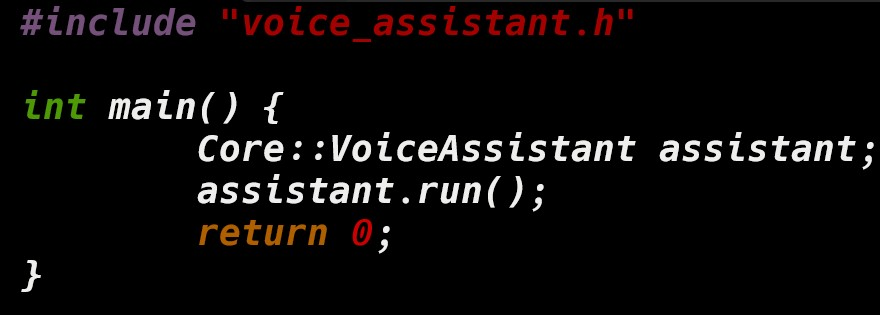
\includegraphics[scale=0.7]{main.jpg}
	\caption{Точка входа в программную систему}
	\label{fig:main.cpp}
\end{figure}

При создании объекта assistant вызывается конструктор класса VoiceAssistant на рисунке \ref{fig:constructor_VoiceAssistant}

\begin{figure}[H]
	\centering
	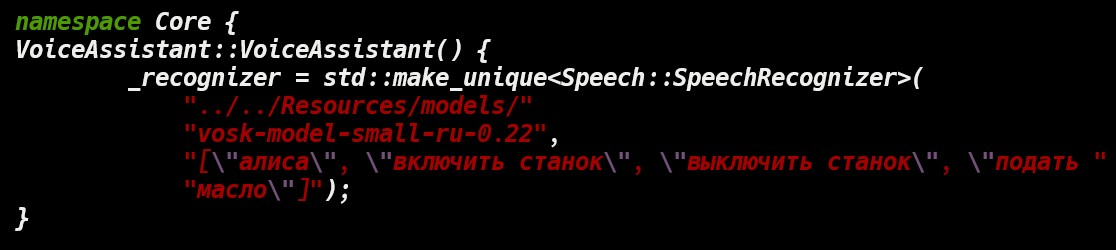
\includegraphics[scale=0.7]{constructor_VoiceAssistant.jpg}
	\caption{Конструктор VoiceAssistant}
	\label{fig:constructor_VoiceAssistant}
\end{figure}

Конструктор класса VoiceAssistant:
\begin{itemize}
 	\item загружается модель распознавания речи Vosk для русского языка;
	\item настраивается ограниченный набор фраз, которые ассистент сможет распознавать.
\end{itemize}

Это повышает точность, так как система не пытается распознать произвольную речь, а ждет только указанные команды.

Затем созданный объекта вызывает метод run() который представлен на рисунке \ref{fig:run_VoiceAssistant}.

\begin{figure}[H]
	\centering
	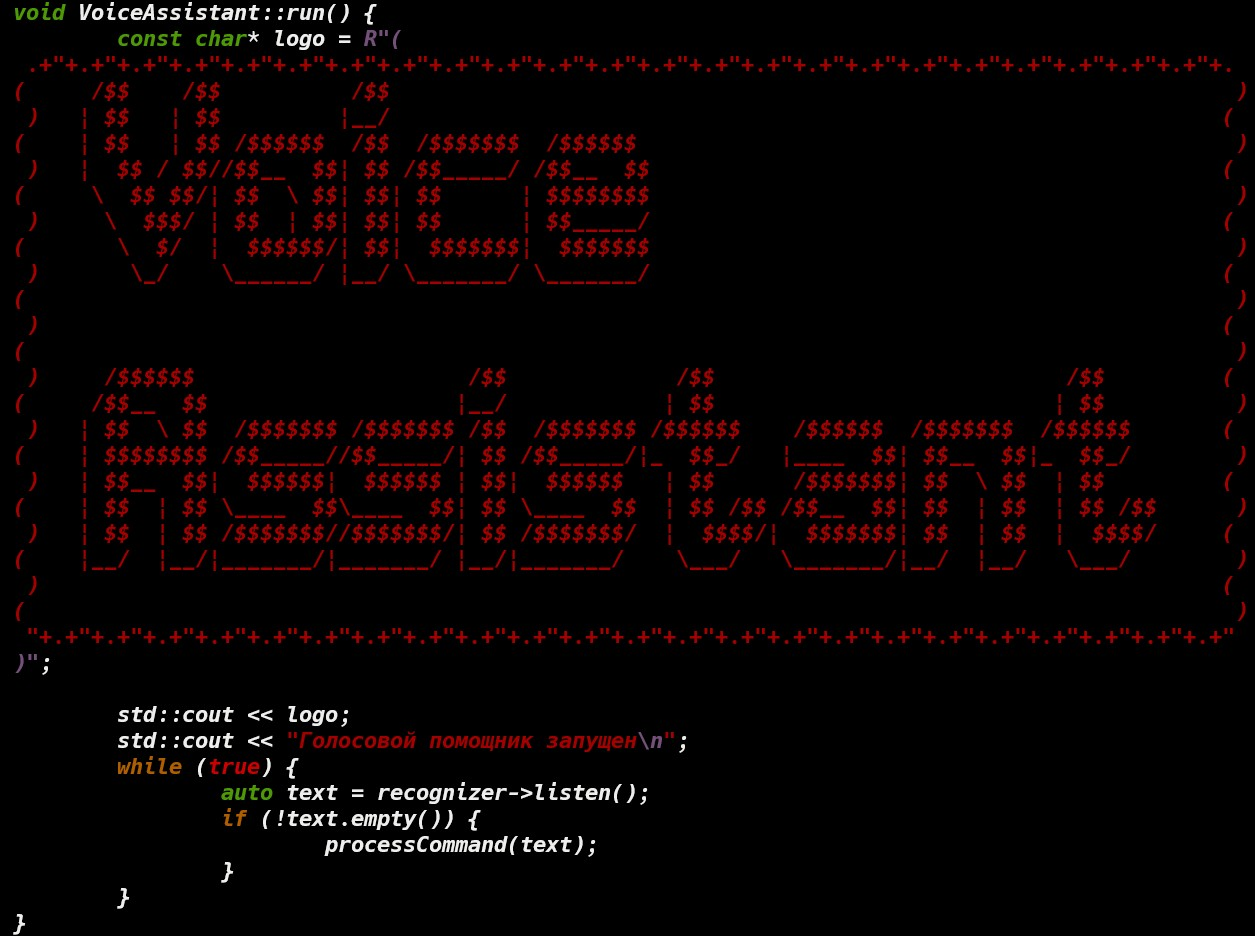
\includegraphics[scale=0.6]{run_VoiceAssistant.jpg}
	\caption{Метод run() класса VoiceAssistant}
	\label{fig:run_VoiceAssistant}
\end{figure}

Метод VoiceAssistant::run() обеспечивает запуск и непрерывную работу голосового ассистента. В начале работы выводится ASCII-графика в виде стилизованного логотипа. Сразу после отображения логотипа программа выводит текстовое сообщение "Голосовой помощник запущен". Основная функциональность реализована через бесконечный цикл, в котором есть объект который создан через конструктор показанный на рисунке \ref{fig:constructor_SpeechRecognizer}.

\begin{figure}[H]
	\centering
	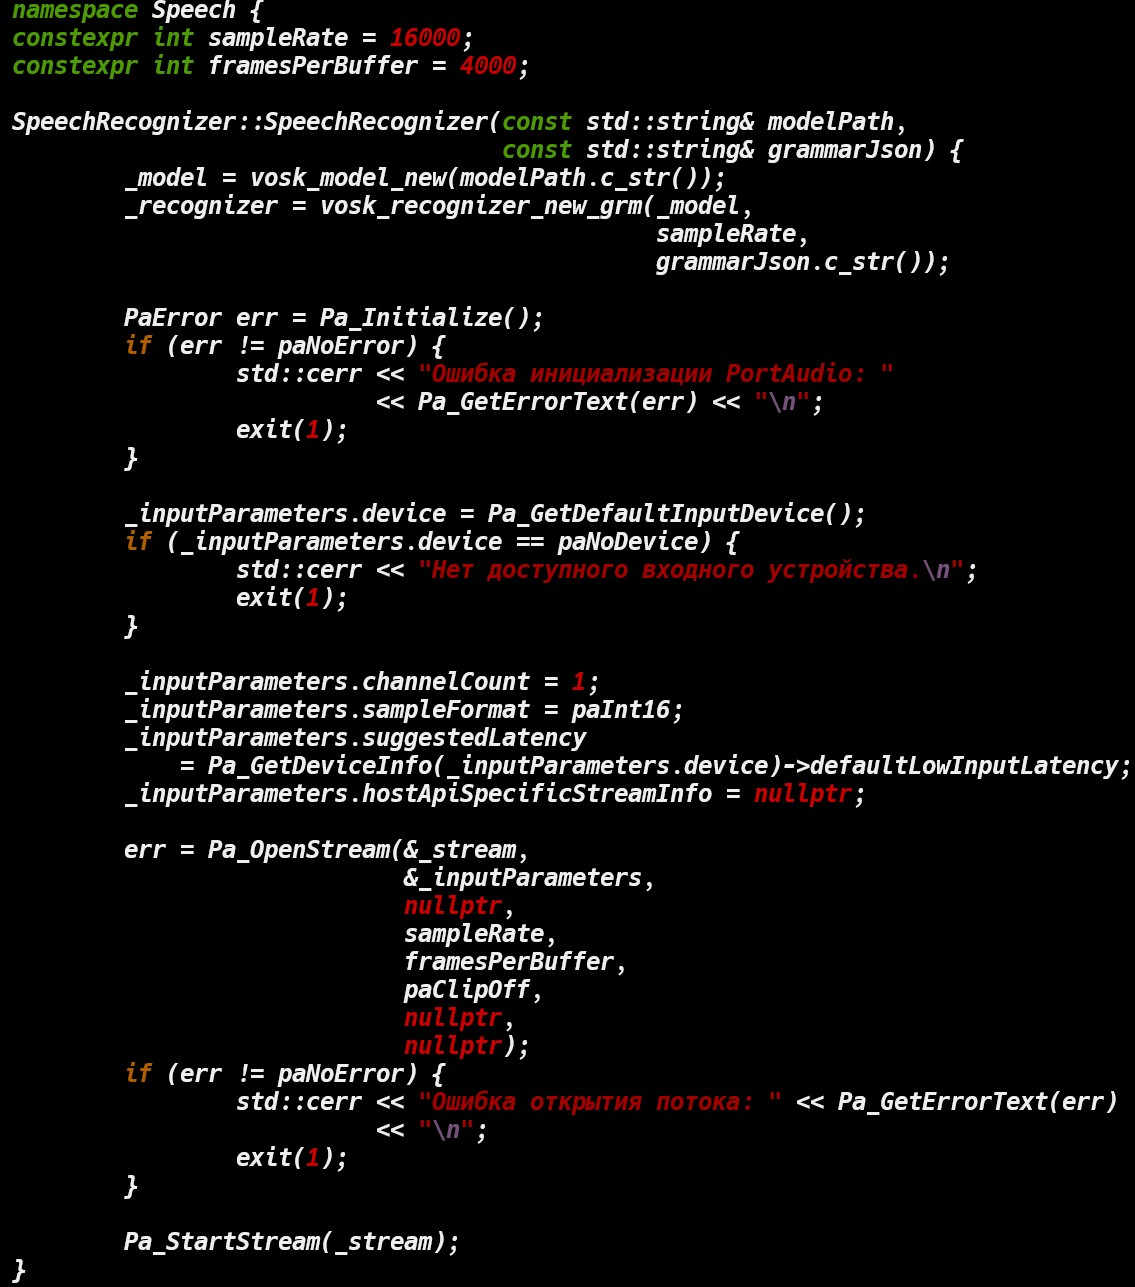
\includegraphics[scale=0.5]{constructor_SpeechRecognizer.jpg}
	\caption{Конструктор SpeechRecognizer}
		\label{fig:constructor_SpeechRecognizer}
\end{figure}
и в котором непрерывно происходит захват аудиопотока через метод listen() представленном на рисунке \ref{fig:listenSpeechRecognizer}.

\begin{figure}[H]
	\centering
	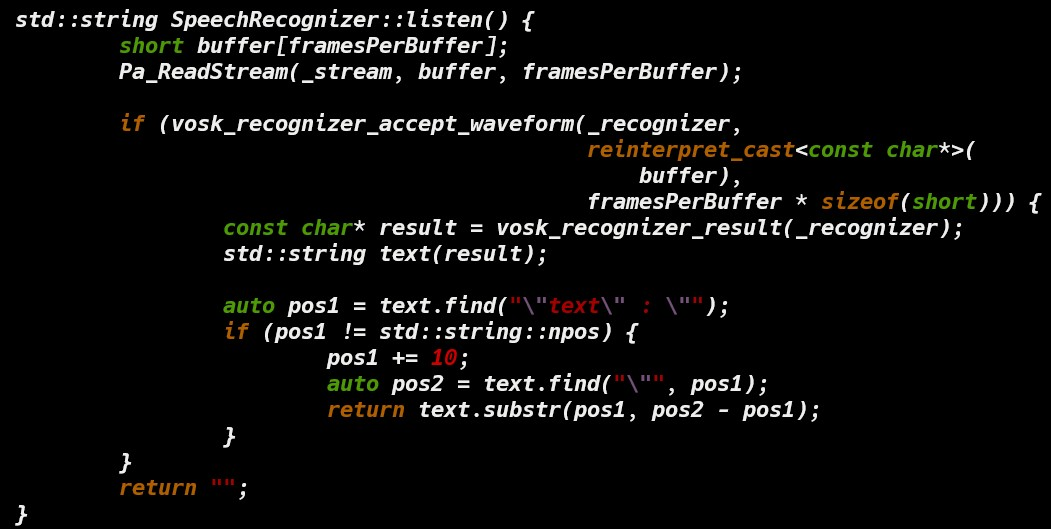
\includegraphics[scale=0.8]{listenSpeechRecognizer.jpg}
	\caption{Метод listen() класса SpeechRecognizer}
	\label{fig:listenSpeechRecognizer}
\end{figure}

Данные метод реализует процесс захвата и обработки аудиоданных для распознавания речи. В начале работы создается буфер размером framesPerBuffer для хранения аудиосэмплов в 16-битном формате. С помощью функции Pa\_ReadStream осуществляется чтение аудиопотока из микрофона, при этом данные записываются в подготовленный буфер. Полученные аудиоданные передаются в распознаватель Vosk через функцию vosk\_recognizer\_accept\_waveform, где происходит их преобразование в текстовый формат.

Если распознавание прошло успешно, функция vosk\_recognizer\_result возвращает результат в виде JSON-строки, содержащей распознанный текст. Из этой строки извлекается непосредственно текстовая часть между полями \string"text\string" : \string" и закрывающей кавычкой. Для этого используется поиск позиций соответствующих подстрок и последующее выделение нужного фрагмента. Если текст успешно извлечен, он возвращается как результат работы метода. В случае неудачного распознавания или отсутствия текста в результате возвращается пустая строка.

Таким образом, метод обеспечивает непрерывный цикл захвата аудио, его преобразование в текст и извлечение распознанных фраз из структуры результата, возвращая их для дальнейшей обработки в системе.

Условие if (!text.empty()) анализирует, содержит ли объект text какую-либо распознанную речевую фразу. Если проверка проходит успешно, это означает, что пользователь произнес осмысленную команду, и система переходит к её обработке, вызывая функцию processCommand(text). Данная логика работы наглядно представлена на рисунке \ref{fig:processCommand_VoiceAssistant}.

\begin{figure}[H]
	\centering
	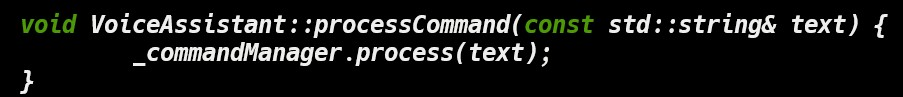
\includegraphics[scale=0.8]{processCommand_VoiceAssistant.jpg}
	\caption{Метод processCommand()  класса VoiceAssistant}
	\label{fig:processCommand_VoiceAssistant}
\end{figure}

Метод processCommand() выполняет передачу распознанной голосовой команды в менеджер команд для дальнейшей обработки. Он принимает текстовую строку с распознанной речью и у объекта созданного через конструктор который представлен на рисунке \ref{fig:constructor_CommandManager}.


\begin{figure}[H]
	\centering
	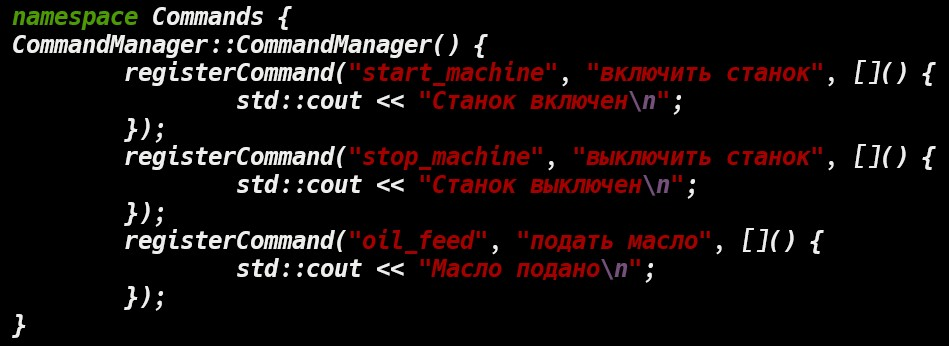
\includegraphics[scale=0.8]{constructor_CommandManager.jpg}
	\caption{Конструктор класса CommandManager}
	\label{fig:constructor_CommandManager}
\end{figure}

Конструктор CommandManager при создании объекта регистрирует три голосовые команды для управления оборудованием через метод registerCommand который представлен на рисунке \ref{fig:registerCommand_CommandManager}.

\begin{figure}[H]
	\centering
	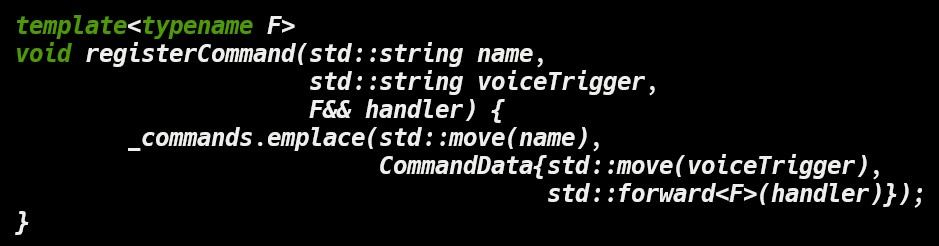
\includegraphics[scale=0.8]{registerCommand_CommandManager.jpg}
	\caption{Метод registerCommand()  класса CommandManager}
	\label{fig:registerCommand_CommandManager}
\end{figure}

Метод registerCommand добавляет новую команду в систему управления. Он принимает три параметра: техническое имя команды, голосовую фразу-триггер и обработчик команды. При вызове метод сохраняет команду во внутреннем хранилище commands, связывая между собой имя команды, её голосовой триггер и функцию-обработчик. Техническое имя и голосовой триггер перемещаются в хранилище, а обработчик передается с сохранением категории значения (lvalue или rvalue). Это позволяет регистрировать различные команды с их обработчиками, которые система сможет выполнять при распознавании соответствующих голосовых фраз.

 и после этого созданы объект commandManager вызывает метод process() которые представлен на рисунке \ref{fig:process_CommandManager}.

\begin{figure}[H]
	\centering
	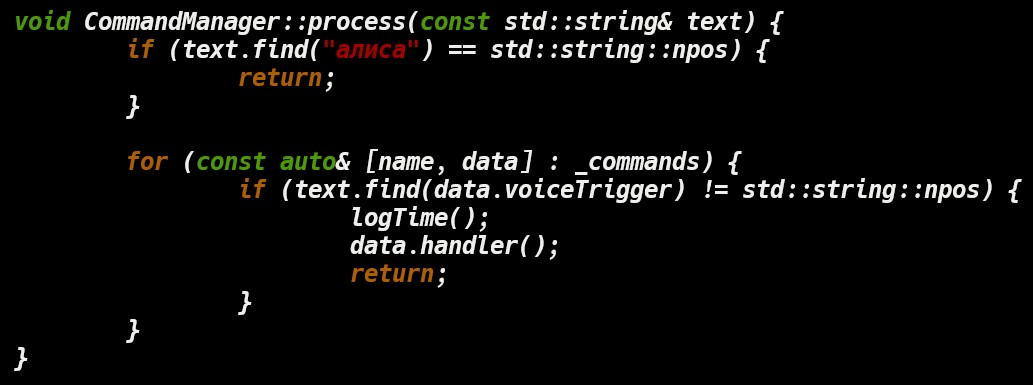
\includegraphics[scale=0.8]{process_CommandManager.jpg}
	\caption{Метод process()  класса CommandManager}
	\label{fig:process_CommandManager}
\end{figure}

Метод CommandManager::process обрабатывает входящую текстовую команду следующим образом. Сначала проверяет, содержит ли текст ключевое слово "алиса" -- если его нет, метод сразу завершает работу без дальнейших действий. Если ключевое слово присутствует, метод перебирает все зарегистрированные команды из хранилища commands и ищет соответствие между текстом команды и сохраненными голосовыми триггерами. При нахождении совпадения метод фиксирует время вызова команды с помощью logTime(), выполняет связанный с командой обработчик handler() и завершает работу. Если ни одна команда не подходит, метод просто завершается без выполнения каких-либо действий. Таким образом, система реагирует только на команды, содержащие слово "алиса" и соответствующие одному из зарегистрированных голосовых шаблонов.

\newpage
